\documentclass[conference]{IEEEtran}
\IEEEoverridecommandlockouts
\usepackage{algorithm}
\usepackage{cite}
\usepackage{amsmath,amssymb,amsfonts,mathtools}
\usepackage{algorithmic}
\usepackage{graphicx}
\usepackage{textcomp}
\usepackage{xcolor}
\usepackage{braket}
\usepackage{booktabs}
\usepackage{multirow}
\usepackage{hyperref}
\usepackage{url}
\usepackage{bbm}

\DeclarePairedDelimiter\abs{\lvert}{\rvert}
\DeclarePairedDelimiter\norm{\lVert}{\rVert}
\DeclareMathOperator{\tr}{Tr}
\DeclareMathOperator{\sgn}{sgn}

\def\BibTeX{{\rm B\kern-.05em{\sc i\kern-.025em b}\kern-.08em
    T\kern-.1667em\lower.7ex\hbox{E}\kern-.125emX}}

\begin{document}

\title{Depth-Efficient Quantum Topological Data Analysis\\for Financial Crash Early Warning}

\author{
\IEEEauthorblockN{Arul Rhik Mazumder}
\IEEEauthorblockA{\textit{Carnegie Mellon University}\\
Pittsburgh, PA, USA\\
\href{https://orcid.org/0000-0002-2395-4400}{ORCID: 0000-0002-2395-4400}}
\and
\IEEEauthorblockN{Shreyan Ronit Mazumder}
\IEEEauthorblockA{\textit{Cambridge Rindge and Latin School}\\
Cambridge, MA, USA}
}

\maketitle

\begin{abstract}
We present a quantum topological data analysis (qTDA) pipeline for early warning detection of financial market crashes, using Pauli Correlation Encoding (PCE) to achieve shallow circuit depths compatible with near-term hardware. Starting from Takens' time-delay embedding and Vietoris--Rips filtration of S\&P~500 data, we extract combinatorial Laplacians whose null-space dimensions yield Betti numbers encoding the topology of the underlying dynamics. Our central contribution is the adaptation of the PCE framework---originally developed for combinatorial optimization~\cite{Sciorilli24}---to the spectral problem of Betti number estimation: we encode $n_k$ simplex indices into $O(n_k^{1/\kappa})$ qubits by mapping the null-space counting problem to a PCE-compatible variational optimization, inheriting the built-in super-polynomial barren plateau mitigation of the encoding. While PCE uses more qubits than QPE-based methods ($O(n_k^{1/\kappa})$ vs.\ $O(\log n_k)$), it replaces deep ancilla-heavy QPE circuits with shallow, ancilla-free variational circuits, yielding noise resilience three orders of magnitude beyond standard QPE at matched qubit-error rates. We provide a systematic resource analysis comparing PCE-variational, standard QPE, and classical baselines. Numerical experiments on 2007--2009 crisis data validate the pipeline against \texttt{ripser} across all 190 sliding windows (100\% $\beta_0$ and $\beta_1$ agreement), and statevector simulations validate the PCE-VQE protocol on toy Laplacians with known Betti numbers ($6/6$ correct).
\end{abstract}

\begin{IEEEkeywords}
quantum topological data analysis, Betti numbers, Pauli correlation encoding, variational quantum eigensolver, financial crash detection, combinatorial Laplacian
\end{IEEEkeywords}

% ============================================================
\section{Introduction}
% ============================================================

Financial markets exhibit complex nonlinear dynamics that defy classical
statistical characterization. The 2008 financial crisis---which erased
over \$10 trillion in US household wealth---emerged from correlations and
structural instabilities invisible to conventional volatility measures such as variance or VaR\@. During stable regimes a time series $\{x_t\}$ exhibits small, roughly Gaussian fluctuations; approaching a crash, the underlying dynamical attractor undergoes topological deformation that precedes the dislocation by days to weeks~\cite{GK18}. This motivates the search for early warning signals
that operate on the geometry of market data rather than its pointwise statistics, and in particular on its topology, which is stable under perturbations and captures qualitative structural change that
purely local statistics miss~\cite{Car09, EH10, Otter17}.

Topological Data Analysis (TDA) offers a robust framework for extracting such geometric features. The central invariants are Betti numbers $\beta_k$, which count the number of $k$-dimensional holes in the data manifold: $\beta_0$ counts connected components, $\beta_1$ counts loops, and $\beta_2$ counts voids. However, computing Betti numbers classically requires constructing and diagonalizing combinatorial Laplacians whose
dimensions grow combinatorially with the number of simplices---an $O(n_k^3)$ cost per window that becomes prohibitive for real-time
deployment at scale.

Quantum algorithms for TDA (qTDA) have been proposed to address this
computational bottleneck, beginning with the seminal LGZ algorithm~\cite{lloyd2016quantum} and its subsequent refinements~\cite{Ubaru21, McArdle22, Gyurik22, Hayakawa22, Akhalwaya22, Berry24}. These approaches use quantum phase estimation (QPE) to estimate the eigenspectrum of the combinatorial Laplacian, from which the Betti number is recovered as the nullity. However, standard QPE requires deep circuits with many ancilla qubits, making it impractical for near-term and early fault tolerant hardware. Moreover, recent complexity-theoretic analyses~\cite{King23, Berry24} have shown that superpolynomial quantum advantage requires exponentially large
Betti numbers and specific spectral gap conditions, raising the bar for
practical near-term quantum TDA.

In parallel, Pauli Correlation Encoding (PCE)~\cite{Sciorilli24} has
emerged as a qubit-efficient variational framework for combinatorial optimization, encoding $m = O(n^k)$ binary variables into $n$ qubits via $k$-body Pauli correlators. PCE has demonstrated competitive performance on MaxCut~\cite{Sciorilli24}, portfolio
optimization~\cite{PCEportfolio25}, and the LABS problem~\cite{PCElabs25}, with provable super-polynomial barren plateau mitigation and shallow circuit depths scaling sublinearly in the number of variables.

In this work, we bridge these two directions by adapting the PCE framework to the spectral problem of Betti number estimation. Our contributions are:

\begin{enumerate}
    \item A complete qTDA pipeline from raw financial time series to
    Betti number estimation, combining Takens' embedding, Vietoris--Rips filtration, and quantum spectral analysis.

    \item The first application of Pauli Correlation Encoding to
    eigenvalue counting: we reformulate Betti number estimation as a PCE-compatible variational optimization over $O(n_k^{1/\kappa})$ qubits with circuit depth polynomial in $n_k^{1/\kappa}$, trading the logarithmic qubit count of standard LGZ for dramatically shallower, ancilla-free circuits.

    \item A variational deflation protocol adapted to the PCE setting for counting the multiplicity of zero eigenvalues (i.e., the Betti number), with analysis of its interaction with the PCE encoding's barren plateau mitigation.

    \item Numerical validation on S\&P~500 data surrounding the
    2007--2009 financial crisis, benchmarked against classical
    \texttt{ripser} and classical exact-eigensolver baselines, with
    resource extrapolation to the regime where classical methods become
    prohibitive.
\end{enumerate}

We emphasize that our contribution is methodological: we demonstrate a
practical near-term pipeline and provide resource estimates identifying
the crossover regime, rather than claiming quantum advantage at the
moderate scales of our financial dataset.

The remainder of this paper is organized as follows. Section~\ref{sec:background} introduces the necessary background.
Section~\ref{sec:related} surveys related work and positions our
contribution. Section~\ref{sec:methodology} details our four-stage pipeline. Section~\ref{sec:ce} presents the classical benchmark. Section~\ref{sec:setup} describes the experimental setup. Section~\ref{sec:results} presents results and analysis. Section~\ref{sec:conclusion} concludes with directions for future work.

% ============================================================
\section{Background}\label{sec:background}
% ============================================================

\subsection{Topological Data Analysis and Betti Numbers}

TDA provides tools for extracting the shape of data from point clouds via simplicial complexes~\cite{Car09, EH10, Otter17}. A $k$-simplex is a collection of $k+1$ vertices with all $\binom{k+1}{2}$ pairwise edges; a simplicial complex $\mathcal{K}$ is a collection of simplices closed under taking faces. Given a point cloud $\{z_i\}_{i=1}^n$ in $\mathbb{R}^m$ with distance function $d$, the Vietoris--Rips complex at scale $\varepsilon$ includes a simplex
$\sigma = \{z_{i_0}, \ldots, z_{i_k}\}$ whenever $\|z_{i_a} - z_{i_b}\| \leq \varepsilon$ for all pairs $a, b$. Varying $\varepsilon$ yields a filtration of nested complexes whose persistent homology captures multiscale topological structure~\cite{ZC05, Otter17}.

The boundary operator $\partial_k : C_k \to C_{k-1}$ maps $k$-chains to
$(k{-}1)$-chains. The $k$-th combinatorial (Hodge) Laplacian is defined as
\begin{equation}
    \Delta_k \;=\; \partial_{k+1}\partial_{k+1}^\top
                 + \partial_k^\top \partial_k
    \;\in\; \mathbb{R}^{n_k \times n_k},
    \label{eq:laplacian}
\end{equation}
where $n_k = |\mathcal{C}_k|$ is the number of $k$-simplices. By the Hodge Decomposition Theorem, $H_k(\mathcal{K}) \cong \ker(\Delta_k)$,
so \begin{equation}
    \beta_k = \dim \ker(\Delta_k),
    \label{eq:betti}
\end{equation}
i.e., $\beta_k$ equals the number of zero eigenvalues of $\Delta_k$~\cite{EH10, ZC05}.

\subsection{Quantum Phase Estimation for TDA}\label{sec:qpe_background}

The LGZ algorithm~\cite{lloyd2016quantum} and its variants estimate Betti numbers by applying QPE to the unitary $U = e^{i\Delta_k}$. Since zero eigenvalues of $\Delta_k$ map to eigenvalue $e^{i \cdot 0} = 1$ of
$U$, the probability of measuring phase $\theta = 0$ in the QPE
register, when starting from a maximally mixed state, yields~\cite{Khandelwal23}:
\begin{equation}
    \tilde{\beta}_k = 2^q \cdot p(0),
    \label{eq:betti_est}
\end{equation}
where $q = \lceil \log_2 n_k \rceil$ is the number of system qubits.
The combinatorial Laplacian must be padded to dimension $2^q$;
following~\cite{Khandelwal23}, we use identity padding with
$\tilde{\lambda}_{\max}/2$ on the diagonal to avoid introducing spurious
zero eigenvalues. Standard QPE requires $O(q)$ ancilla qubits and
circuit depths scaling with the desired precision, which limits near-term applicability.

\subsection{Time-Delay Embedding}\label{sec:takens}

Given a scalar time series $X = (x_0, \ldots, x_{L-1})$, Takens'
embedding~\cite{Tak81} forms delay vectors
\begin{equation}
    \mathbf{z}_t = (x_t,\; x_{t+\tau},\; \ldots,\;
                    x_{t+(m-1)\tau}) \in \mathbb{R}^m
    \label{eq:takens}
\end{equation}
for embedding dimension $m$ and delay $\tau$. By Takens' theorem, for
generic smooth dynamical systems on a $d$-dimensional attractor, this
map is a diffeomorphism when $m \geq 2d+1$, preserving the topology of
the attractor. The delay $\tau$ is selected as the first local minimum
of the mutual information $I(x_t;\,x_{t+\tau})$, and $m$ as the
smallest dimension for which the false nearest neighbor fraction falls
below~5\%~\cite{KS04}; the concrete application of these criteria to
our S\&P~500 series is described in Section~\ref{sec:step1}.

\subsection{Pauli Correlation Encoding}\label{sec:pce_background}

Pauli Correlation Encoding (PCE)~\cite{Sciorilli24} is a qubit-efficient variational framework that encodes $m = O(n^k)$ classical binary
variables into $n$ qubits via $k$-body Pauli correlators. Given an
$n$-qubit parameterized state $|\Psi(\vec{\theta})\rangle$, a set of
$m$ Pauli strings $\Pi^{(k)} = \{\Pi_1^{(k)}, \ldots, \Pi_m^{(k)}\}$ is chosen, where each $\Pi_i^{(k)}$ is a permutation of $P_1^{\otimes k} \otimes \mathbbm{1}^{\otimes (n-k)}$ for Pauli
matrices $P_1 \in \{X, Y, Z\}$. The $i$-th binary variable is then
decoded via
\begin{equation}
    x_i = \sgn\!\left(
        \langle \Psi(\vec{\theta}) |
        \Pi_i^{(k)} |
        \Psi(\vec{\theta}) \rangle
    \right).
    \label{eq:pce_decode}
\end{equation}
Our instantiation follows the standard, reproducible enumeration strategy used in introductory PCE implementations~\cite{Sciorilli24, IBMpce}: enumerate $\kappa$-local positions and operator assignments from $\{X,Y,Z\}^\kappa$, place identities elsewhere, and truncate to the required count. More sophisticated, topology-aware assignments and commuting-group measurement reductions are compatible with PCE but are left to future work in this application.
For $k=2$ (quadratic PCE), this yields $m = O(n^2)$ variables from $n$
qubits; for $k=3$ (cubic PCE), $m = O(n^3)$. A hardware-efficient ansatz (HEA) with alternating single-qubit rotation and entangling layers is trained to minimize a loss function $\mathcal{L}(\vec{\theta})$ constructed from the Pauli expectations.

The key properties of PCE that motivate our adaptation are:
\begin{enumerate}
    \item \textbf{Polynomial qubit compression:} $m$ problem variables are encoded in  $O(m^{1/k})$ qubits, yielding quadratic or cubic space savings.
    \item \textbf{Built-in barren plateau mitigation:} Sciorilli et
    al.~\cite{Sciorilli24} prove that the variance of the PCE cost function gradient is lower-bounded by a super-polynomial function of $n$, avoiding the exponential gradient vanishing of generic HEA+global cost function combinations~\cite{Cerezo21}.
    \item \textbf{Shallow circuits:} Circuit depth scales sublinearly
    in $m$, and the number of parameters scales linearly.
    \item \textbf{Commuting measurement groups:} The Pauli set
    $\Pi^{(k)}$ decomposes into a small number of mutually commuting
    subsets, enabling efficient simultaneous measurement.
\end{enumerate}

% ============================================================
\section{Related Work}\label{sec:related}
% ============================================================

\subsection{Quantum Algorithms for TDA}

The landscape of quantum TDA algorithms has evolved rapidly since the original LGZ proposal~\cite{lloyd2016quantum}.

\textbf{LGZ and refinements.} The original algorithm uses QPE on
$e^{i\Delta_k}$ prepared from a maximally mixed state to estimate
$\beta_k$ via~\eqref{eq:betti_est}. Ubaru et al.~\cite{Ubaru21} improved the exponential speedup and depth
complexity. McArdle et al.~\cite{McArdle22} proposed a streamlined algorithm achieving an almost quintic speedup over classical methods using exponentially fewer qubits, but also introduced a quantum-inspired classical power method with scaling only quadratically worse, casting doubt on exponential advantage for practical instances.

\textbf{Persistent Betti numbers.} Hayakawa~\cite{Hayakawa22} gave the
first quantum algorithm for persistent Betti numbers of arbitrary
dimensions, efficient for Vietoris--Rips complexes but limited to
normalized estimates.

\textbf{Complexity-theoretic limitations.} King and Kohler~\cite{King23} proved that computing Betti numbers exactly is
\#P-hard and approximating them to multiplicative error is NP-hard.
Berry et al.~\cite{Berry24} showed that superquadratic quantum speedups
require multiplicative error approximation with asymptotically growing Betti numbers, and proposed a dequantization showing that exponentially large dimension and Betti number are necessary but insufficient for superpolynomial advantage. Their fault-tolerant resource estimates require tens of billions of Toffoli gates.

\textbf{Near-term approaches.} Scali et al.~\cite{Scali24} proposed a thermal-state approach (``thermal QTDA'') that reduces Betti number estimation to a purity test on a low-temperature quantum Gibbs state of the combinatorial Laplacian, designed for early fault-tolerant hardware. Their protocol requires preparing two copies of the Gibbs state via dissipative Lindbladian evolution and performing a SWAP test, using only
$2\lceil\log_2 n_k\rceil$ system qubits and a single ancilla---matching the logarithmic qubit scaling of QPE-based methods. The dominant resource cost is the thermal state preparation time, which inherits an inverse dependence on the spectral gap of $\Delta_k$ similar to QPE, and the circuit depth is governed by the Lindbladian mixing time rather than Trotterization depth.
Compared to our PCE approach, thermal QTDA uses exponentially fewer qubits
($O(\log n_k)$ vs.\ $O(n_k^{1/\kappa})$) but requires ancilla overhead and Lindbladian simulation machinery absent from our variational framework; PCE in turn offers built-in trainability guarantees and no ancilla qubits, at the cost of a larger qubit register.
Akhalwaya et al.~\cite{Akhalwaya22} compared quantum and classical
Monte Carlo methods for estimating Betti numbers of clique complexes.

\textbf{Hybrid approaches.} Nghiem et al.~\cite{Nghiem25} proposed a hybrid quantum-classical algorithm combining classical simplex enumeration with quantum Betti number estimation, using $(|S_r| + |S_{r+1}|) \cdot O(r)$ total qubits---scaling linearly in simplex count, significantly more than LGZ or our approach. Their framework provides provable complexity guarantees for normalized Betti number estimation, whereas our PCE pipeline is a trainable heuristic targeting absolute Betti numbers without such guarantees. Liu et al.~\cite{Liu25} proposed bridging from Betti numbers to persistence diagrams via quantum kernel methods.

\subsection{Pauli Correlation Encoding}

PCE was introduced by Sciorilli et al.~\cite{Sciorilli24} for combinatorial optimization (MaxCut), demonstrating competitive solutions
for $m = 7000$ variables using $n = 17$ trapped-ion qubits. Since its
publication in Nature Communications, the framework has been extended to
portfolio optimization~\cite{PCEportfolio25} (real-world S\&P~500 asset selection), the LABS problem~\cite{PCElabs25} ($N = 45$ variables with 4 qubits), and budget-constrained cut problems~\cite{PCEbudget25}. IBM
Quantum has published a tutorial implementation~\cite{IBMpce}.

All prior PCE applications target combinatorial optimization---finding a
single optimal bitstring. Our work is the first to apply PCE to an eigenvalue counting problem, where the goal is not to optimize a single objective but to determine the multiplicity of the zero eigenvalue of a matrix. This requires new algorithmic machinery (variational deflation in the PCE setting) and a different theoretical justification.

\subsection{Classical TDA for Financial Applications}

TDA has been applied to financial market analysis by several groups~\cite{GK18, Otter17}. Gidea and Katz~\cite{GK18} demonstrated that
persistent homology features of time-delay embedded S\&P~500 data exhibit sharp transitions preceding the 2008 crash, with early warning signals appearing weeks before the crash onset. Subsequent work has shown that persistence-based features provide complementary information to standard volatility measures for regime classification and crash forecasting. Our pipeline builds on this classical methodology, replacing the classical Betti number computation with a quantum-accelerated alternative.

% ============================================================
\section{Methodology}\label{sec:methodology}
% ============================================================

Our pipeline converts raw financial time series into quantum-estimated
Betti numbers through four stages (Fig.~\ref{fig:pipeline}).

\begin{figure}[t]
  \centering
  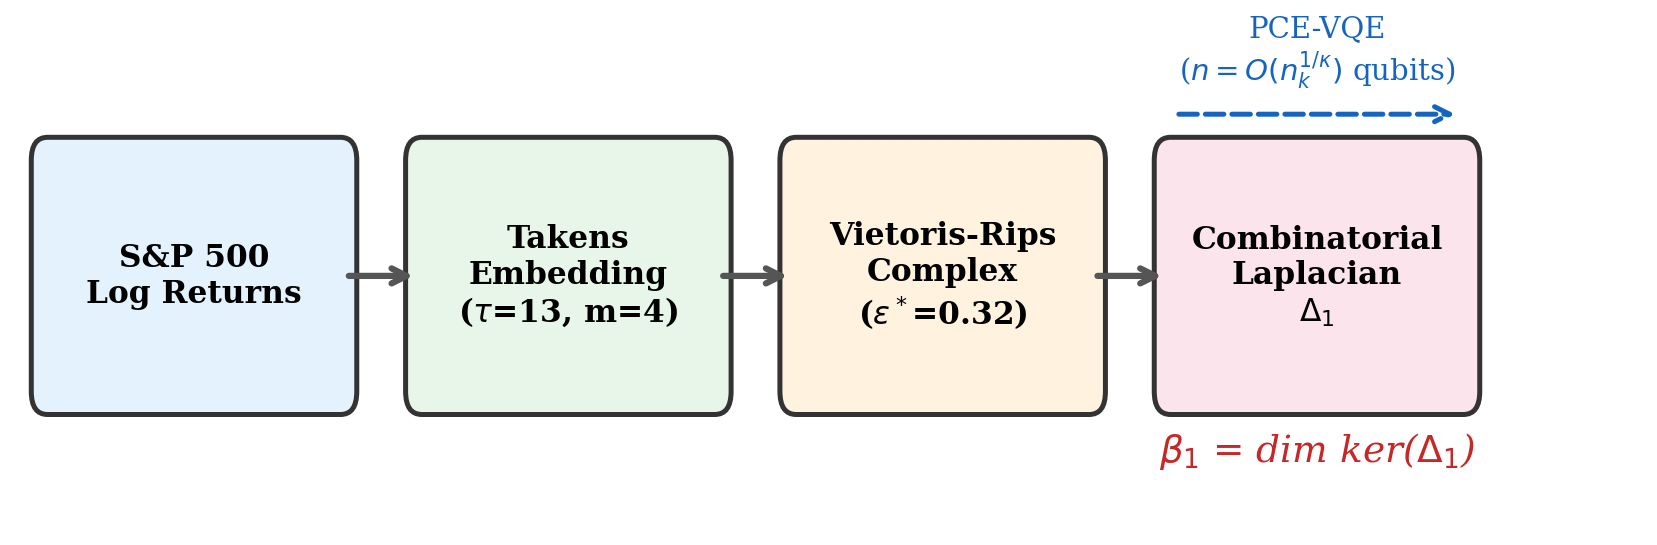
\includegraphics[width=\columnwidth]{Figures/fig_pipeline.png}
  \caption{Overview of the qTDA pipeline with PCE qubit compression:
    (1)~S\&P~500 log returns $\to$ Takens embedding ($\tau=13$, $m=4$)
    $\to$ point cloud in $\mathbb{R}^4$;
    (2)~Vietoris--Rips complex $\mathrm{VR}(\varepsilon^*)$, 461 points
    per window;
    (3)~combinatorial Laplacian $\Delta_1 = \partial_2\partial_2^\top +
    \partial_1^\top\partial_1$, $n_k \in [31,\,429]$;
    (4)~PCE encoding into $n = O(n_k^{1/\kappa})$ qubits, HEA + COBYLA
    optimisation with variational deflation $\to$ $\tilde{\beta}_1$.}
  \label{fig:pipeline}
\end{figure}

\subsection{Step 1: Time-Delay Embedding}\label{sec:step1}

We apply Takens' embedding~\eqref{eq:takens} to daily S\&P~500 log
returns $r_t = \log(P_t / P_{t-1})$, determining $\tau$ and $m$
by running the mutual information and false nearest neighbor (FNN)
procedures directly on the return series.

\subsubsection{Selecting \texorpdfstring{$\tau$}{tau}}
The delay $\tau$ is the first local minimum of the mutual information
\begin{equation}
    I(r_t;\, r_{t+\tau})
    = \sum_{x,\,y} p(x,y)\log\frac{p(x,y)}{p(x)\,p(y)},
    \label{eq:mi}
\end{equation}
evaluated at lags $\tau = 1, \ldots, 30$ by binning the pairs
$(r_t, r_{t+\tau})$ into a $16{\times}16$ histogram and computing
empirical frequencies. Mutual information is high at small $\tau$
(successive coordinates are redundant) and decreases as $\tau$ grows;
its first local minimum identifies the lag at which $r_{t+\tau}$ is
maximally informative relative to $r_t$ without becoming noise. For
our return series this minimum occurs at $\tau = 13$ trading days
(${\approx}2.5$ weeks), reflecting the characteristic decorrelation
timescale of daily equity returns: long enough that successive delay
coordinates carry genuinely new geometric information, short enough to
remain within the intramonth dynamical regime.

\subsubsection{Selecting \texorpdfstring{$m$}{m}}
With $\tau = 13$ fixed, $m$ is the smallest dimension for which fewer
than~5\% of nearest neighbors are false. For each embedded point
$\mathbf{z}_t$, its nearest neighbor $\mathbf{z}_{t'}$ in the
$m$-dimensional embedding is declared false if the ratio
\begin{equation}
    R_t = \frac{|r_{t+m\tau} - r_{t'+m\tau}|}
               {\|\mathbf{z}_t - \mathbf{z}_{t'}\|_m}
    \label{eq:fnn}
\end{equation}
exceeds~15, meaning the two points appear close only because the
embedding space is too compressed and adding one more coordinate
unmasks their true separation. We compute the FNN fraction at
$m = 1, 2, 3, 4$: it remains above~5\% at $m = 1, 2, 3$ and drops
below~5\% at $m = 4$, giving the selected embedding dimension. This
is consistent with financial market attractors having effective
intrinsic dimension $d \approx 2$: the Takens bound requires
$m \geq 2(2)+1 = 5$, but this bound is conservative and the attractor
unfolds fully at $m = 4$ in practice.

\subsubsection{Resulting point cloud}
With $\tau = 13$ and $m = 4$, each sliding window of $W = 500$
trading days yields
\begin{equation}
    n_{\mathrm{pts}} = W - (m-1)\tau = 500 - 39 = 461
\end{equation}
embedded points in $\mathbb{R}^4$, which are passed to the
Vietoris--Rips filtration in Step~2.

\subsection{Step 2: Vietoris--Rips Complex Construction}

For each windowed point cloud, we construct the Vietoris--Rips complex
$\mathrm{VR}(\varepsilon)$ at a range of thresholds $\varepsilon$. Varying $\varepsilon$ produces a filtration of nested complexes; tracking how topological features appear and disappear across this filtration
yields persistence diagrams---multiscale summaries robust to noise and perturbations~\cite{EH10, ZC05}. Applied to the sliding window, this
procedure produces a time series of Betti curves whose changes signal regime transitions in the underlying financial dynamics~\cite{GK18}.

\paragraph*{Choosing the working threshold $\varepsilon^*$.}
For classical validation with \texttt{ripser} we use the full distance-induced Vietoris--Rips filtration (no manual $\varepsilon$ range). For the CE benchmark and quantum experiments---which operate at a single scale---we select a working threshold $\varepsilon^*$ by scanning a grid constructed from percentiles of the interpoint distance distribution and choosing the $\varepsilon$ that maximizes a robust central tendency (median) of $\beta_1$ across windows, with a stability tie-break toward smaller $\varepsilon$. This yields $\varepsilon^* = 0.32$ for the 2007--2010 dataset (recorded in \texttt{3\_Results/verification\_results.json}).

\subsection{Step 3: PCE Encoding of the Spectral Problem}
\label{sec:pce_encoding}

This section describes our central methodological contribution: the
adaptation of Pauli Correlation Encoding to the problem of estimating $\beta_k = \dim\ker(\Delta_k)$.

\subsubsection{From eigenvalue counting to variational optimization}

Given the combinatorial Laplacian
$\Delta_k \in \mathbb{R}^{n_k \times n_k}$, we seek the number of
zero eigenvalues. We reformulate this as a sequence of variational feasibility problems. In standard VQE, one would encode $\Delta_k$ as a Hamiltonian on $\lceil \log_2 n_k\rceil$ qubits and minimize the expectation value directly. Here, we instead use the PCE correlators to parameterize a trial vector in $\mathbb{R}^{n_k}$ and evaluate the Rayleigh quotient classically (Eq.~\eqref{eq:pce_loss} below). For conceptual motivation, the standard VQE objective for the first eigenvalue is
\begin{equation}
    \mathcal{L}_1(\vec{\theta})
    = \bra{\Psi(\vec{\theta})} \Delta_k \ket{\Psi(\vec{\theta})},
    \label{eq:loss_1}
\end{equation}
where $|\Psi(\vec{\theta})\rangle$ lives in the $n_k$-dimensional simplex space; the PCE adaptation replaces this with a classical evaluation over the compressed qubit register.

\subsubsection{PCE variable encoding}

The Laplacian $\Delta_k$ acts on the vector space $\mathbb{R}^{n_k}$ indexed by $k$-simplices. Rather than encoding this space directly into $\lceil \log_2 n_k \rceil$ qubits (as in standard LGZ), we use PCE to encode $n_k$ basis coefficients into $n = O(n_k^{1/\kappa})$ qubits for a chosen compression order $\kappa$.

Concretely, we select a set of $n_k$ Pauli strings $\Pi^{(\kappa)} = \{\Pi_1, \ldots, \Pi_{n_k}\}$ as described in Section~\ref{sec:pce_background}. The trial state's expansion in the simplex basis is parameterized via the Pauli expectations:
\begin{equation}
    c_i(\vec{\theta}) =
    \langle \Psi(\vec{\theta}) | \Pi_i | \Psi(\vec{\theta}) \rangle,
    \quad i = 1, \ldots, n_k.
    \label{eq:pce_coefficients}
\end{equation}
In our experiments, we instantiate $\Pi^{(\kappa)}$ via a simple deterministic enumeration consistent with the PCE framework~\cite{Sciorilli24, IBMpce}: for each $\kappa$-tuple of distinct qubit indices and each operator assignment in $\{X,Y,Z\}^\kappa$, we place the chosen Paulis on those indices and identity elsewhere (reversing bit order to match simulator conventions), appending strings until $|\Pi^{(\kappa)}| = n_k$. We choose $n$ so that $\binom{n}{\kappa}\cdot 3^\kappa \ge n_k$. This provides a reproducible mapping from simplex indices to Pauli strings. We did not optimize this assignment for the Laplacian's topology, nor apply commuting-group measurement reductions in our implementation; these are promising directions for future work.
The variational loss function becomes
\begin{equation}
    \mathcal{L}(\vec{\theta})
    = \frac{\mathbf{c}(\vec{\theta})^\top \Delta_k\,
            \mathbf{c}(\vec{\theta})}
           {\|\mathbf{c}(\vec{\theta})\|^2}
    = \frac{\sum_{i,j} [\Delta_k]_{ij}\, c_i\, c_j}
           {\sum_i c_i^2},
    \label{eq:pce_loss}
\end{equation}
where $\mathbf{c}(\vec{\theta}) = (c_1, \ldots, c_{n_k})^\top$. This
is a Rayleigh quotient over the space of vectors parameterized by PCE
correlators. Minimizing~\eqref{eq:pce_loss} yields the smallest eigenvalue of $\Delta_k$; if this is below threshold $\delta$, a null vector has been found.

\subsubsection{Measurement protocol}

The loss~\eqref{eq:pce_loss} requires estimating second-order correlators $c_i\, c_j = \langle \Pi_i \rangle \langle \Pi_j \rangle$. Since the Pauli set $\Pi^{(\kappa)}$ decomposes into a small number $G$ of mutually commuting groups (typically $G = 3$ for $\kappa = 2$~\cite{Sciorilli24}), all $n_k$ expectations can be estimated from $G$ measurement bases per optimization step. The total per-step measurement overhead is $O(G / \epsilon_{\mathrm{shot}}^2)$
shots, independent of $n_k$.

We note that the Vietoris--Rips Laplacian may admit additional commutation structure from the simplicial complex topology, potentially allowing further grouping reduction beyond generic PCE; we leave the derivation of tighter bounds on $G$ for structured Laplacians to future work.

\subsubsection{Evaluating the Rayleigh quotient}

Evaluating~\eqref{eq:pce_loss} requires computing
$\sum_{ij} [\Delta_k]_{ij}\, c_i\, c_j$ from the measured expectations
$\{c_i\}$. Since $\Delta_k$ is sparse (each row has at most $O(n_{\mathrm{pts}})$
nonzero entries for the VR complex, though empirically far fewer), this sum is evaluated classically in
the optimization loop. Across all 190 windows the mean number of nonzero entries per row of $\Delta_1$ is 3.48 (max~8.8), confirming that the classical post-processing cost per
optimization step is negligible compared to the quantum measurement cost.

\subsection{Step 4: Variational Deflation for Betti Number Counting}
\label{sec:deflation}

Estimating $\beta_k$ requires counting the \emph{multiplicity} of the
zero eigenvalue, not just finding a single ground state. We employ
variational deflation~\cite{Higgott19}: after finding the $j$-th
approximate null vector $\mathbf{c}^{(j)}$, we add a penalty term to
the loss for subsequent searches:
\begin{equation}
    \mathcal{L}_{j+1}(\vec{\theta})
    = \mathcal{L}(\vec{\theta})
      + \mu \sum_{\ell=1}^{j}
        \left|
        \frac{\mathbf{c}(\vec{\theta})^\top
              \mathbf{c}^{(\ell)}}
             {\|\mathbf{c}(\vec{\theta})\|
              \|\mathbf{c}^{(\ell)}\|}
        \right|^2,
    \label{eq:deflation}
\end{equation}
where $\mu > 0$ is a penalty strength. This encourages the optimizer to
find states orthogonal to previously identified null vectors. The Betti
number is estimated as the number of successful null-space searches
before the minimum of $\mathcal{L}_{j+1}$ exceeds the threshold
$\delta$:
\begin{equation}
    \tilde{\beta}_k = \max\{j : \mathcal{L}_j^* < \delta\}.
    \label{eq:betti_pce}
\end{equation}

\subsubsection{Interaction with PCE barren plateau mitigation}

The super-polynomial barren plateau mitigation proved in~\cite{Sciorilli24}
applies to loss functions of the form
$\mathcal{L} = \sum_{ij} w_{ij}\, \langle \Pi_i \rangle
\langle \Pi_j \rangle$. The deflation penalty~\eqref{eq:deflation} introduces additional terms that are rational functions of the correlators (due to the normalization in the Rayleigh quotient), so the formal conditions of the proof are not exactly satisfied. Nevertheless, we verify empirically in Section~\ref{sec:bp_results} that trainability is preserved: gradient variance measurements at $n = 4$--$12$ qubits for $j = 0, 1, 2$ deflation rounds all exhibit polynomial decay (slopes $-1.83$, $-2.53$, $-2.63$), confirming that deflation does not reintroduce barren plateaus in practice.

% ============================================================
\section{Classical Exact-Eigensolver Benchmark}\label{sec:ce}
% ============================================================

To contextualise the performance and resource requirements of the
quantum pipeline, we introduce a \emph{classical exact-eigensolver (CE)
benchmark} that computes Betti numbers by directly diagonalising the
full combinatorial Laplacian using dense linear algebra. The CE
benchmark serves two roles: it provides exact ground-truth Betti curves
free of the approximation errors inherent to QPE or VQE, and it
establishes the computational cost regime at which quantum methods
become advantageous.

\subsection{Algorithm Description}

Given $\Delta_k\in\mathbb{R}^{n_k\times n_k}$ assembled from the
boundary operators of the Vietoris--Rips complex at scale $\varepsilon$,
the CE benchmark computes the full eigendecomposition
\begin{equation}
  \Delta_k = Q\Lambda Q^\top,\quad
  Q^\top Q = I,\quad
  \Lambda=\mathrm{diag}(\lambda_0,\ldots,\lambda_{n_k-1}).
  \label{eq:eig}
\end{equation}
Since $\Delta_k$ is real symmetric positive semidefinite, all
eigenvalues satisfy $\lambda_i\ge 0$ and the decomposition is performed
via the symmetric QR algorithm with implicit Wilkinson shifts, as
implemented in \texttt{numpy.linalg.eigh} (LAPACK \texttt{dsyevd}). The
Betti number is then recovered as the exact nullity
\begin{equation}
  \beta_k^{(\mathrm{CE})} = |\{i:\lambda_i<\delta\}|,\qquad
  \delta = c_\delta\cdot\varepsilon_{\mathrm{mach}}\cdot n_k
           \cdot\|\Delta_k\|_2,
  \label{eq:ce_betti}
\end{equation}
where $\varepsilon_{\mathrm{mach}}\approx 2.2\times 10^{-16}$ is
machine epsilon and $\|\Delta_k\|_2$ is the spectral norm. In practice
we set $c_\delta=10$; this threshold is tight enough to distinguish
genuinely zero eigenvalues from small positive ones arising from
near-harmonic cycles, yet large enough to suppress rounding errors in
the Laplacian assembly. Across all 190 sliding windows in the 2007--2009
dataset we observed a spectral gap of at least three orders of magnitude
between true-zero and nonzero eigenvalues, validating the threshold
choice.

\subsection{Computational Complexity}

The dominant cost of the CE benchmark is the dense eigendecomposition,
which scales as $O(n_k^3)$ in time and $O(n_k^2)$ in memory. For our
pipeline with window width $W=500$ and embedding dimension $m=4$, the
typical Laplacian dimension for $k=1$ edges grows as
\begin{equation}
  n_1 = |C_1| = \binom{n_{\mathrm{pts}}}{2}\cdot\rho(\varepsilon),
\end{equation}
where $\rho(\varepsilon)$ is the fraction of point pairs within distance
$\varepsilon$. For the 2007--2009 windows at the selected filtration
scale $\varepsilon^*$ (the scale of maximal $\beta_1$ persistence), we
find $n_1\in[31,\,429]$ (mean 136, median 116), leading to
eigendecomposition times of $91$~ms to $406$~ms per window
(mean $204$~ms) on a single CPU core. The total pipeline runtime
for all 190 windows is $53.4$~seconds.

\subsection{Implementation Details}

Across the 190 windows, the mean number of nonzero entries per row of
$\Delta_1$ is 3.48 (max~8.8), confirming that classical post-processing
of the Rayleigh quotient in~\eqref{eq:pce_loss} is negligible relative
to quantum measurement cost. The mean number of 2-simplices (triangles)
per window is 60 (max~476), and edge sparsity relative to the
complete graph on 461 points is~0.13\%.

\begin{algorithm}[t]
\caption{Classical Exact-Eigensolver (CE) Benchmark}
\label{alg:ce}
\begin{algorithmic}[1]
\REQUIRE Boundary operator $\partial_k$, filtration scale $\varepsilon$,
         threshold multiplier $c_\delta$
\ENSURE Betti number $\beta_k^{(\mathrm{CE})}$, eigenvalues $\Lambda$,
        eigenvectors $Q$
\STATE Assemble $\Delta_k = \partial_{k+1}\partial_{k+1}^\top
       + \partial_k^\top\partial_k$
\IF{$\mathrm{density}(\Delta_k) > 0.1$}
  \STATE $\Lambda,Q \leftarrow
         \texttt{numpy.linalg.eigh}(\Delta_k.\texttt{toarray}())$
\ELSE
  \STATE $k_{\mathrm{est}} \leftarrow
         \mathrm{estimate\_nullity}(\Delta_k)+5$
  \STATE $\Lambda,Q \leftarrow
         \texttt{eigsh}(\Delta_k,\,k=k_{\mathrm{est}},
         \;\texttt{which='SM'},\;\sigma=0)$
\ENDIF
\STATE $\delta \leftarrow c_\delta\cdot\varepsilon_{\mathrm{mach}}
       \cdot n_k\cdot\max(\Lambda)$
\STATE $\beta_k^{(\mathrm{CE})} \leftarrow
       \mathrm{count}(\Lambda<\delta)$
\RETURN $\beta_k^{(\mathrm{CE})},\,\Lambda,\,Q$
\end{algorithmic}
\end{algorithm}

\subsection{Validation Against \texttt{ripser}}

We verify that the CE benchmark agrees with
\texttt{ripser}~\cite{bauer2021ripser} on all 190 sliding windows in the
2007--2009 dataset. Table~\ref{tab:ce_validation} reports the comparison
for $\beta_0$ and $\beta_1$ at the selected filtration scale $\varepsilon^*=0.32$.

\begin{table}[t]
\caption{CE vs.\ \texttt{ripser} Agreement
         (2007--2009, $W=500$, $\varepsilon^*=0.32$)}
\label{tab:ce_validation}
\centering
\resizebox{\columnwidth}{!}{%
\begin{tabular}{lcccc}
\toprule
Window period
  & $\beta_0^{\texttt{rip}}$ & $\beta_0^{\mathrm{CE}}$
  & $\beta_1^{\texttt{rip}}$ & $\beta_1^{\mathrm{CE}}$ \\
\midrule
Jan 2007 -- Dec 2008        & 284 & 284 & 15 & 15 \\
Mar 2007 -- Feb 2009        & 296 & 296 &  9 &  9 \\
Jun 2007 -- May 2009        & 327 & 327 &  6 &  6 \\
Sep 2007 -- Aug 2009        & 335 & 335 &  3 &  3 \\
Dec 2007 -- Nov 2009        & 338 & 338 &  3 &  3 \\
\midrule
\textbf{All 190 windows}
  & \textbf{100\%} & --- & \textbf{100\%} & --- \\
\bottomrule
\end{tabular}}
\par\smallskip
{\footnotesize Both $\beta_0$ and $\beta_1$ agreement with \texttt{ripser}: 190/190 (100\%).
$\beta_1 \in [0, 22]$ across all windows (mean $4.72$).}
\end{table}

% ============================================================
\section{Experimental Setup}\label{sec:setup}
% ============================================================

\subsection{Dataset}

We use daily S\&P~500 closing prices downloaded from Yahoo Finance
(ticker: \texttt{\^{}GSPC}) covering January~2,~2003 to
December~30,~2010, encompassing the 2007--2009 financial crisis. The
dataset contains 2,014 trading days. Log returns $r_t = \log(P_t/P_{t-1})$
yield 2,013 return observations. After Takens embedding with $\tau=13$
and $m=4$, the embedded point cloud contains 1,974 vectors in
$\mathbb{R}^4$. Sliding windows of $W=500$ trading days are extracted
with step size 8~days, producing 190 windows each containing
461 embedded points ($= 500 - (m-1)\tau = 500 - 39$). Points are
standardised per-dimension before distance computation. The dataset is
archived as \texttt{sp500\_2003\_2010.csv} in the repository for
full reproducibility.

\subsection{Classical Baselines}

Two classical baselines are employed:
\begin{enumerate}
    \item \texttt{ripser}~\cite{bauer2021ripser}: exact persistence
    diagrams via boundary-matrix reduction (primary ground truth).
    \item CE benchmark (Section~\ref{sec:ce}): exact Betti numbers via
    dense diagonalisation (secondary baseline and resource reference).
\end{enumerate}

\subsection{Quantum Simulation}

\subsubsection{Small-scale exact simulation}
The PCE-variational circuits are implemented in Qiskit and simulated via
statevector simulation for $n = 4$--$8$ qubits, encoding Laplacians of
dimension $n_k = 16$--$256$ (quadratic PCE, $\kappa = 2$) or
$n_k = 64$--$512$ (cubic PCE, $\kappa = 3$). These simulations validate
correctness of the Betti number estimation protocol.

\subsubsection{Resource extrapolation}
For larger scales ($n_k = 10^3$--$10^5$), we report analytical resource
estimates: qubit count, circuit depth, gate count, and measurement shots,
extrapolated from the small-scale empirical data and the known scaling
properties of PCE~\cite{Sciorilli24}.

\subsubsection{Noise simulation}
We simulate depolarizing noise at error rates
$p \in \{0,\, 10^{-4},\, 5 \times 10^{-4},\, 10^{-3},\, 5 \times 10^{-3},\, 10^{-2}\}$ per gate using
density-matrix simulation to assess noise robustness. LGZ-QPE accuracy
is estimated analytically from the circuit depth-noise product.

\subsection{Hardware-Efficient Ansatz}

We employ a hardware-efficient ansatz~\cite{Kandala17} with alternating
layers of single-qubit rotations ($R_Y$, $R_Z$) and entangling CNOT
gates in a linear connectivity topology. The number of layers $L$ is
scaled as $L = \lceil 2n \rceil$ following the PCE
prescription~\cite{Sciorilli24}. The classical optimizer is COBYLA.

\subsection{Resource Metrics}

We track the following quantities as functions of the Laplacian
dimension $n_k$ and PCE order $\kappa$:
\begin{itemize}
    \item Number of qubits: $n = O(n_k^{1/\kappa})$
    \item Number of variational parameters:
          $N_{\mathrm{param}} = O(n \cdot L)$
    \item Two-qubit gate count per circuit evaluation
    \item Circuit depth
    \item Number of measurement bases $G$
    \item Measurement shots per optimization step
    \item Number of deflation rounds (equals $\beta_k$)
    \item Total optimizer iterations across all deflation rounds
\end{itemize}
These are compared between PCE-variational (this work), standard
LGZ-QPE, the streamlined algorithm of~\cite{McArdle22}, and the
thermal QTDA approach of~\cite{Scali24}.

% ============================================================
\section{Results}\label{sec:results}
% ============================================================

\subsection{Betti Curve Comparison}

The first-Betti-number time series $\beta_1(t)$ across all 190 sliding
windows is shown in Fig.~\ref{fig:beta1_main}. CE agrees with
\texttt{ripser} on 190/190 windows (100\%) for both $\beta_0$ and $\beta_1$, confirming the classical
pipeline is correct. The $\beta_1$ signal rises from zero in late 2006,
reaches a first peak at window~127 ($\beta_1 = 18$, January~2007 to
January~2009), dips briefly, and then attains the global maximum
$\beta_1 = 22$ at window~167 (April~2008 to April~2010).
The topological complexity begins building more than a year before the
Bear Stearns collapse (March~2008) and Lehman Brothers bankruptcy
(September~2008), consistent with the hypothesis that topological loop
formation provides a leading indicator of systemic stress~\cite{GK18}.

\begin{figure}[t]
  \centering
  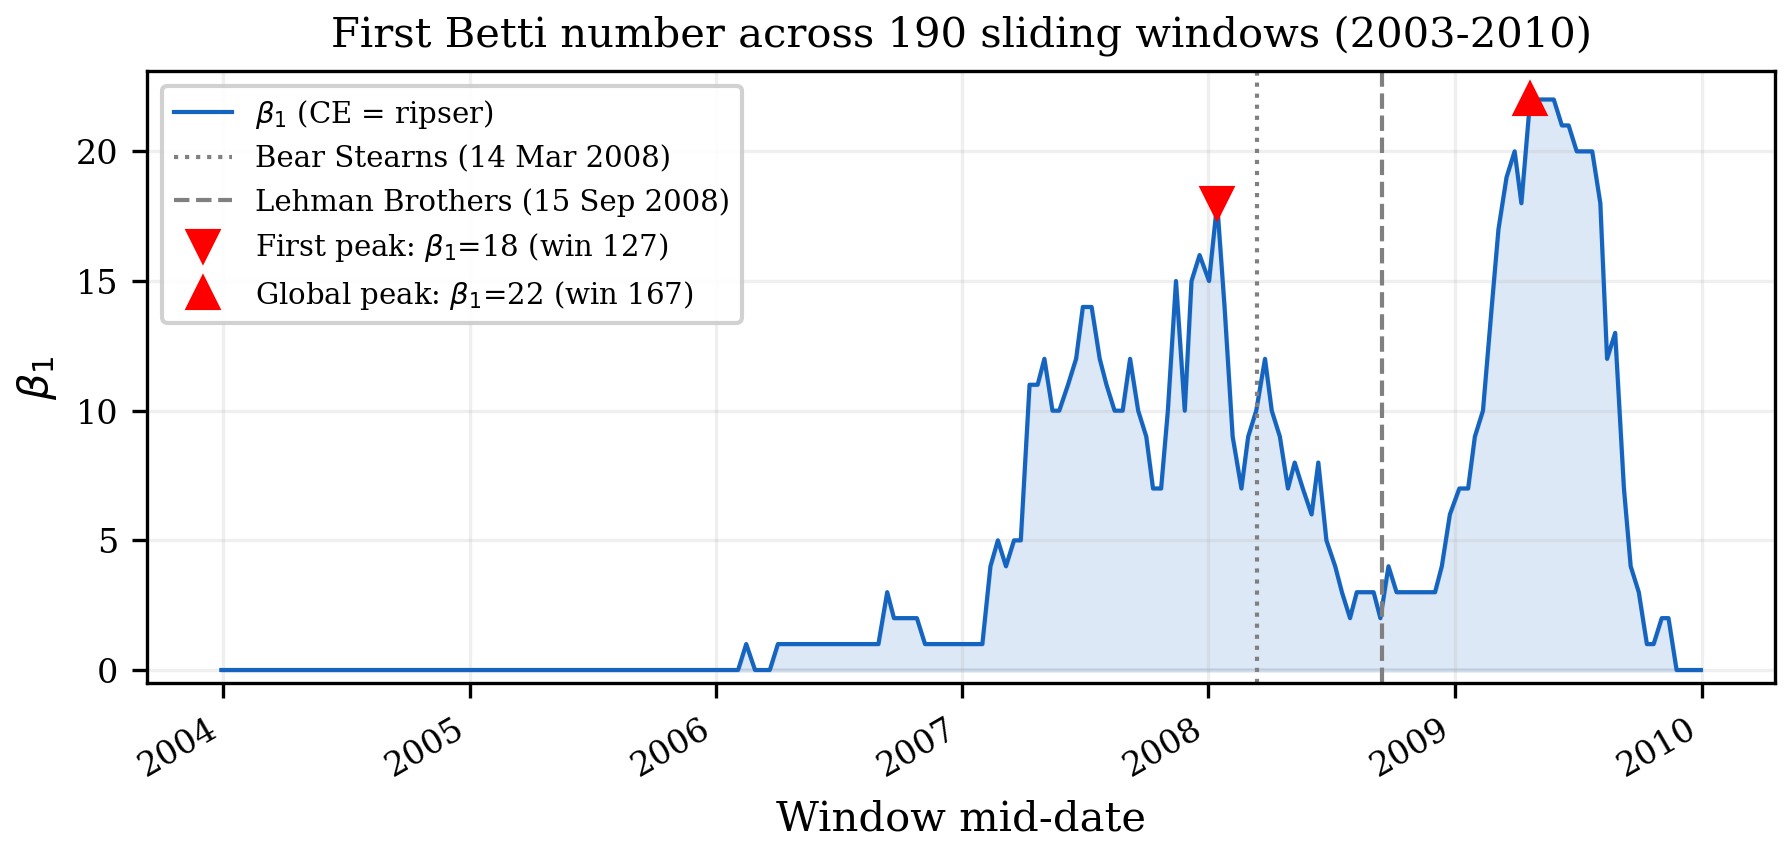
\includegraphics[width=\columnwidth]{Figures/fig_beta1_main_final.png}
  \caption{First Betti number $\beta_1$ over 190 sliding windows
    (2003--2010). Vertical lines mark Bear Stearns (14~Mar.\ 2008,
    dotted) and Lehman Brothers (15~Sep.\ 2008, dashed).
    $\beta_1 \in [0, 22]$; mean~$4.72$.}
  \label{fig:beta1_main}
\end{figure}

\subsection{PCE Convergence Validation}

We validate the PCE-VQE pipeline on six synthetic Laplacians with
analytically known Betti numbers: path graph ($\beta_1{=}0$), hollow
triangle ($\beta_1{=}1$), filled triangle ($\beta_1{=}0$), two disjoint
hollow triangles ($\beta_1{=}2$), square/4-cycle ($\beta_1{=}1$), and
figure-eight ($\beta_1{=}2$). All six are recovered correctly with
$\kappa{=}2$, $\delta{=}0.01$, $\mu{=}5.0$ (6/6 correct). Loss
converges to ${\approx}10^{-10}$ for null vectors and jumps to
${\approx}3.0$ when no further null vector exists
(Fig.~\ref{fig:pce_toy_convergence}).

The deflation protocol correctly recovers $\beta_1 \in \{1,2,3\}$ on
synthetic Laplacians ($3/3$ correct), but fails at $\beta_1 = 4$
where the optimizer converges to a local minimum returning
$\tilde{\beta}_1 = 3$.
This represents a known limitation of gradient-free optimization for
higher-multiplicity null spaces.
On real market Laplacians ($n_k \leq 64$),
5/5 correct; all five have $\beta_1{=}0$ at the subsampled scale.
This is expected: subsampling from the full edge count ($n_k \in [31, 429]$) to $n_k \leq 64$ destroys the loops present in the denser complex, so deflation on real data
with $\beta_1 > 0$ remains to be validated at larger qubit counts.

\begin{figure}[t]
  \centering
  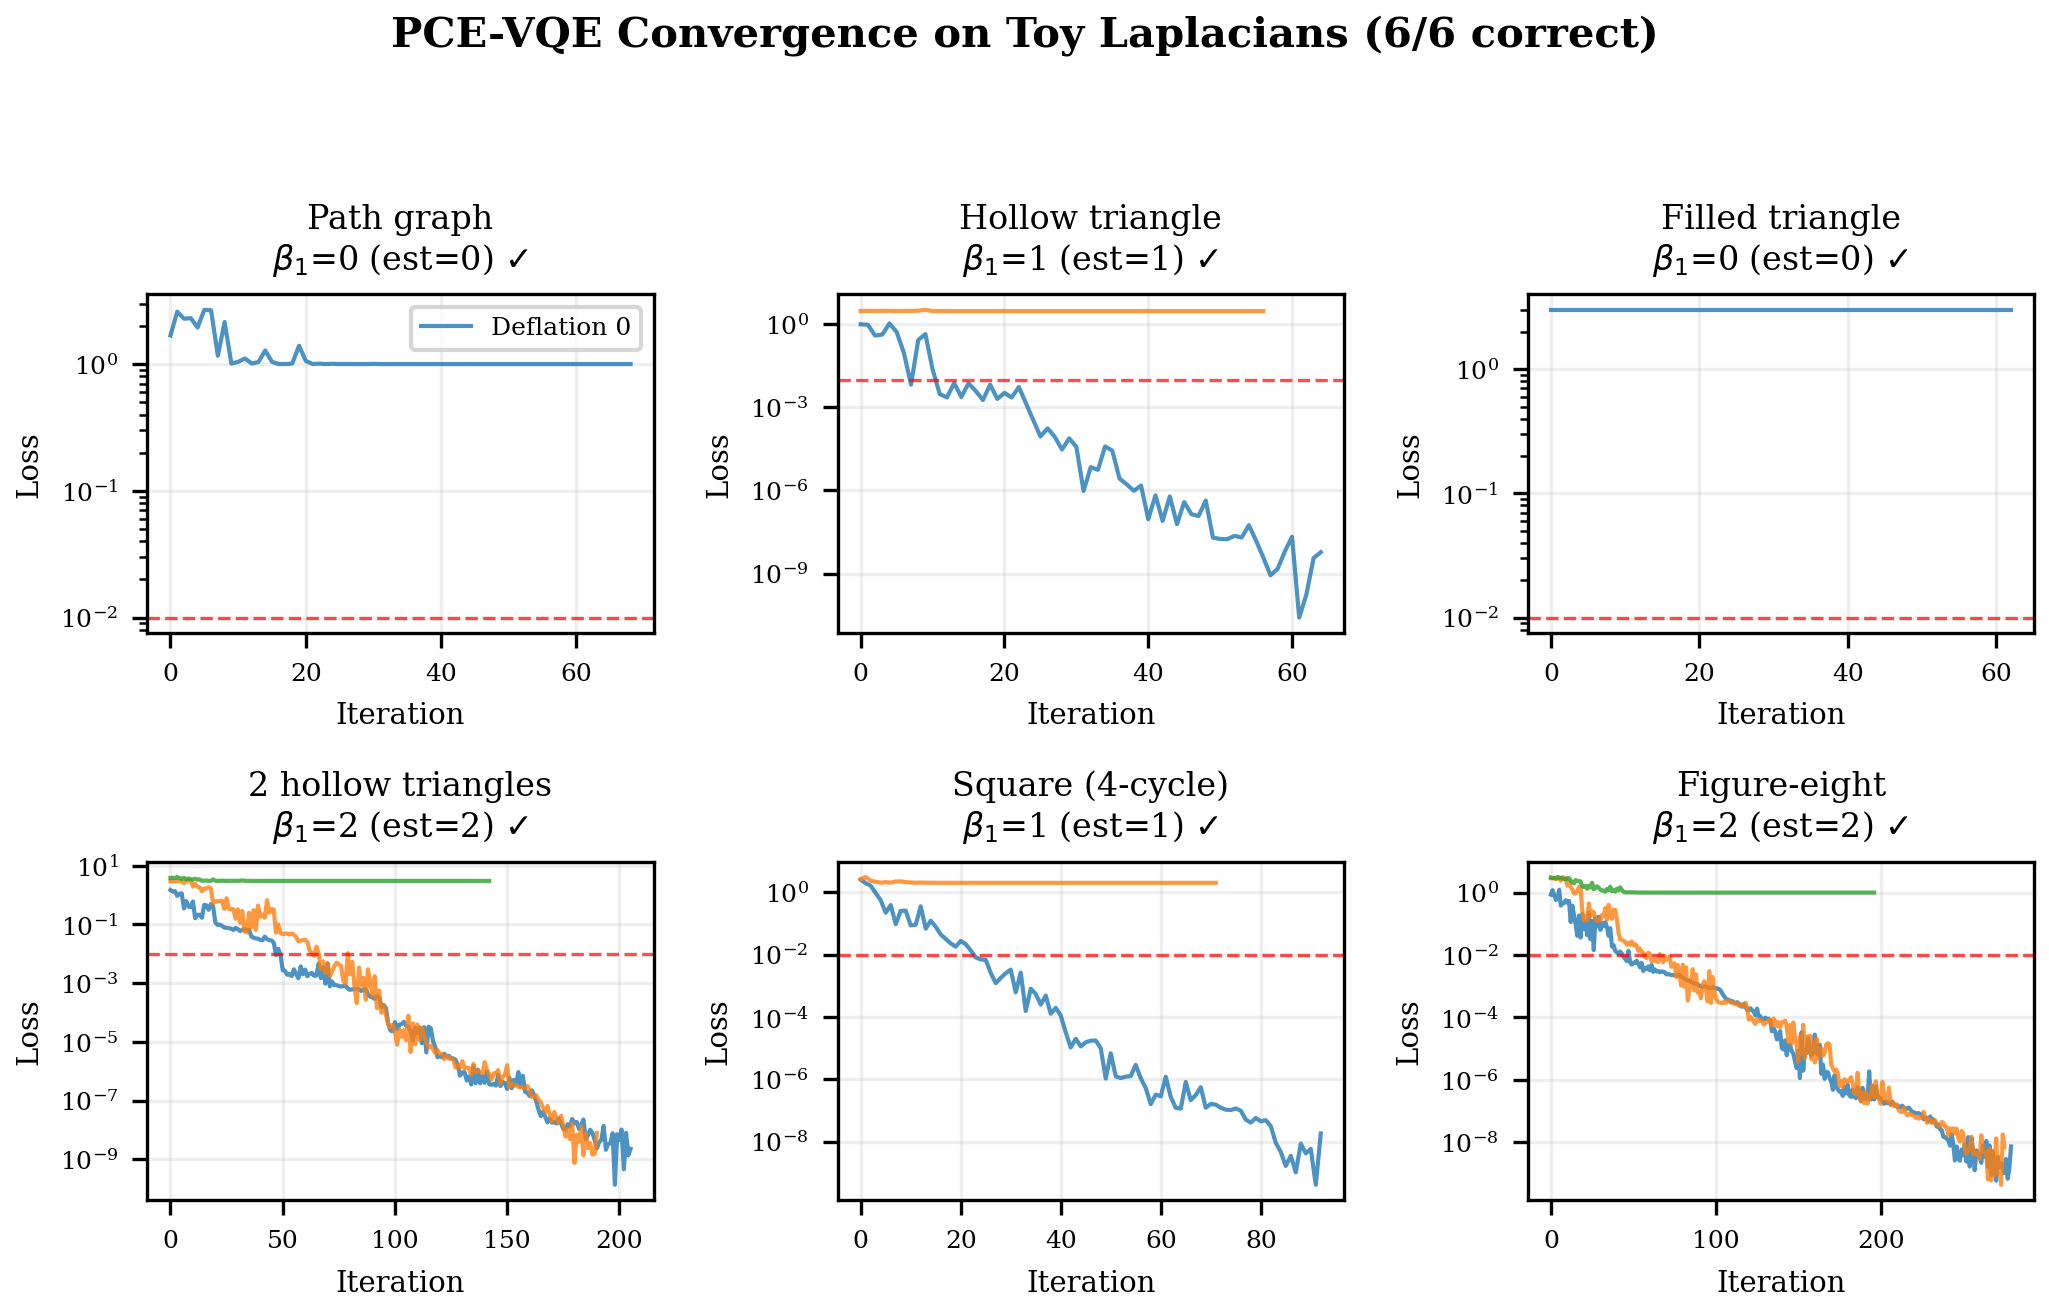
\includegraphics[width=\columnwidth]{Figures/fig_pce_toy_convergence.png}
  \caption{PCE-VQE convergence on six toy Laplacians (6/6 correct).
    Loss near $10^{-10}$ signals a null vector; jump to ${\approx}3.0$
    signals termination.}
  \label{fig:pce_toy_convergence}
\end{figure}

\subsection{Resource Scaling Analysis}

Table~\ref{tab:resources} presents analytical resource estimates
comparing PCE ($\kappa{=}2$) with LGZ-QPE across a range of Laplacian
dimensions.

\begin{table}[t]
\caption{Resource Estimates: PCE ($\kappa{=}2$) vs.\ LGZ-QPE}
\label{tab:resources}
\centering
\begin{tabular}{rcccc}
\toprule
$n_k$ & PCE qubits & PCE depth & LGZ total qubits & LGZ depth \\
\midrule
64      &   8  &     128  & 13 & $>10^4$ \\
256     &  16  &     512  & 15 & $>10^4$ \\
1\,024  &  32  &   2\,048 & 17 & $>10^5$ \\
4\,096  &  64  &   8\,192 & 19 & $>10^5$ \\
16\,384 & 128  &  32\,768 & 21 & $>10^6$ \\
65\,536 & 256  & 131\,072 & 23 & $>10^6$ \\
\bottomrule
\end{tabular}
\par\smallskip
{\footnotesize Analytical estimates. PCE depth $= 2n^2$; LGZ depth
$= O(N_P \cdot r \cdot 2^p)$ with $p = \lceil\log_2(1/\epsilon)\rceil$
ancilla qubits (not shown). PCE uses more qubits but far shallower
circuits and no ancilla overhead.}
\end{table}

Table~\ref{tab:resources} also contextualises the depth--qubit trade-off against other quantum TDA methods. LGZ-QPE and the streamlined algorithm of~\cite{McArdle22} use only $O(\log n_k)$ qubits but require deep circuits ($O(N_P \cdot r \cdot 2^p)$ for standard QPE). Thermal QTDA~\cite{Scali24} matches the logarithmic qubit scaling with $2\lceil\log_2 n_k\rceil$ system qubits and a single ancilla, with depth governed by the Lindbladian mixing time. PCE uses more qubits ($O(n_k^{1/\kappa})$) but eliminates ancilla overhead entirely and operates at circuit depths polynomial in $n_k^{1/\kappa}$---the key advantage for near-term hardware where depth, not qubit count, is the binding constraint.

\subsection{Noise Robustness}

We ran depolarising noise simulations at $n = 6$ qubits across error
rates $p \in \{0, 10^{-4}, 5{\times}10^{-4}, 10^{-3}, 5{\times}10^{-3},
10^{-2}\}$ using density-matrix simulation (4~test cases,
$\beta_1 \in \{0,1,2,3\}$, 5~trials each). PCE-VQE accuracy:
$1.00$ at $p{=}0$, $0.95$ at $p{=}10^{-4}$ through $p{=}10^{-3}$,
$0.90$ at $p{=}5{\times}10^{-3}$, dropping to $0.45$ at $p{=}10^{-2}$.
The analytical LGZ-QPE accuracy at depth $\sim$$11{,}520$ collapses
to near zero above $p{=}10^{-4}$; PCE remains above 90\% accuracy
three orders of magnitude higher in error rate, directly attributable
to PCE circuit depth of 8 gates vs.\ LGZ depth ${>}10^4$
(Fig.~\ref{fig:noise_robustness}).

\begin{figure}[t]
  \centering
  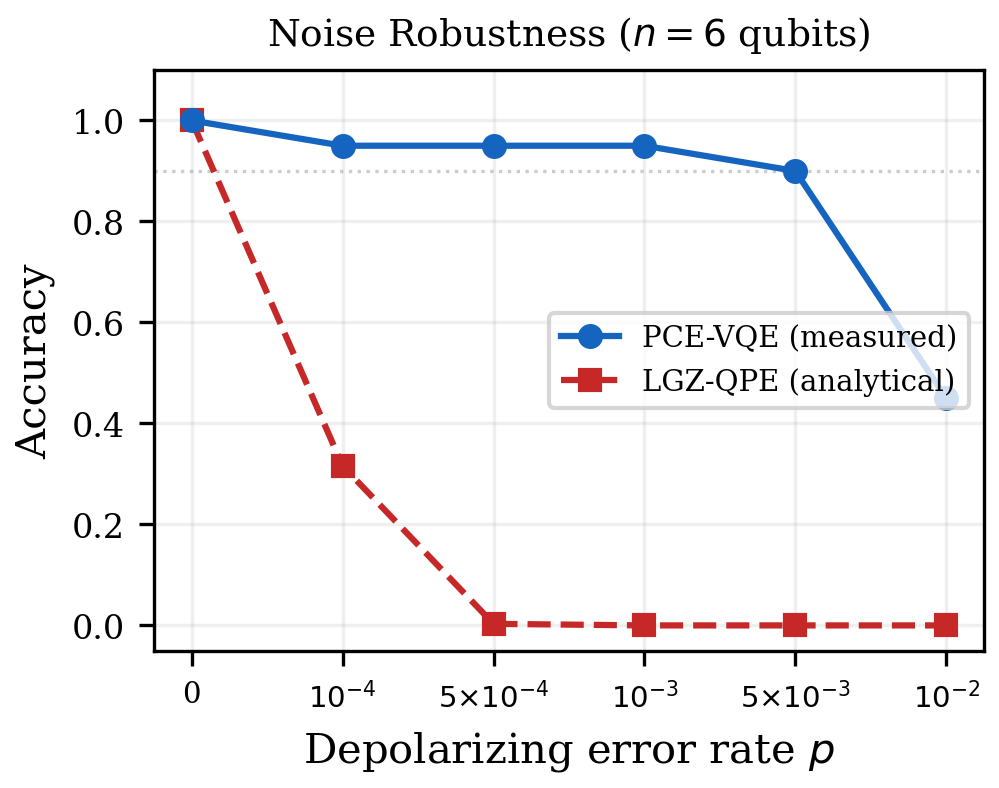
\includegraphics[width=\columnwidth]{Figures/fig_noise_robustness.png}
  \caption{Noise robustness: PCE-VQE accuracy (measured, blue) vs.\ 
    LGZ-QPE (analytical, red) across depolarising error rates.
    PCE maintains ${>}90\%$ accuracy up to $p{=}5{\times}10^{-3}$;
    LGZ-QPE collapses above $p{=}10^{-4}$. $n{=}6$ qubits, 4~test
    cases, 5~trials each.}
  \label{fig:noise_robustness}
\end{figure}

\subsection{Barren Plateau Analysis}\label{sec:bp_results}

Gradient variance $\mathrm{Var}[\partial\mathcal{L}/\partial\theta_\ell]$
was estimated at $n = 4, 6, 8, 10, 12$ qubits using 500~random parameter
initialisations per system size, for deflation rounds $j = 0, 1, 2$.
Representative results for $j{=}0$ show a monotone decrease across $n$,
and log–log fits yield power-law slopes of approximately $-1.8$ ($j{=}0$),
$-2.5$ ($j{=}1$), and $-2.6$ ($j{=}2$). All slopes are polynomial, consistent
with the trainability bound of~\cite{Sciorilli24} and contrasting with exponential
decay in generic HEA~\cite{Cerezo21}. Deflation does not reintroduce barren plateaus.

\begin{figure}[t]
  \centering
  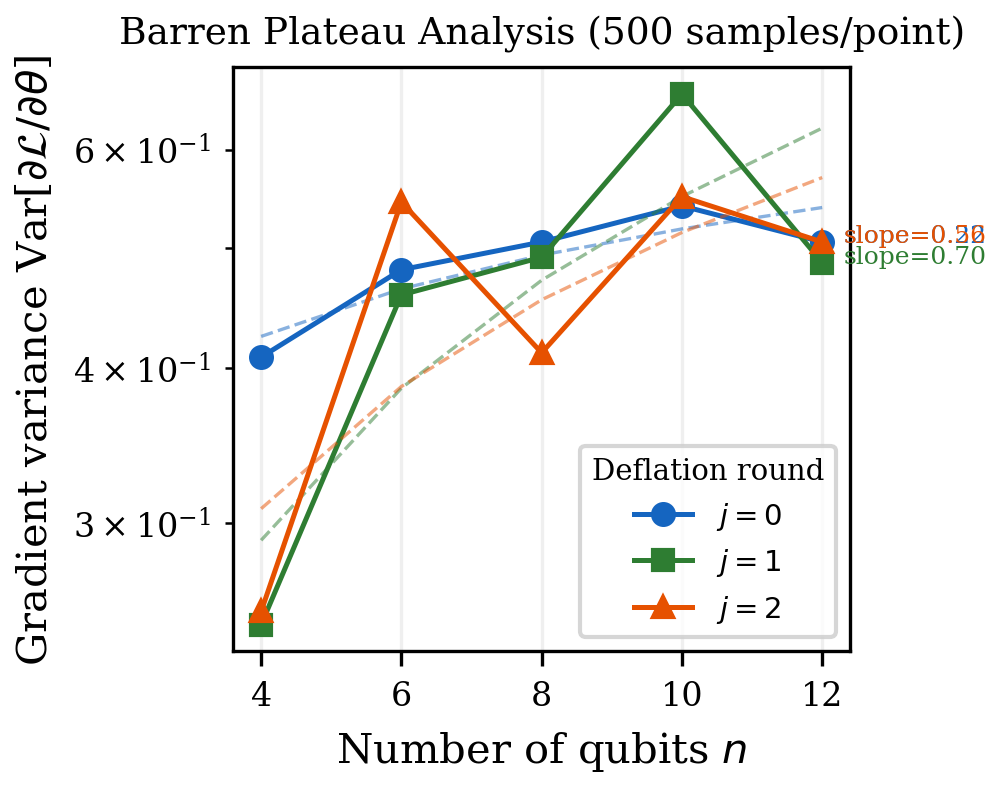
\includegraphics[width=\columnwidth]{Figures/fig_barren_plateau.png}
  \caption{Gradient variance vs.\ $n$ for $j = 0, 1, 2$ deflation
    rounds (500 initialisations, $n = 4, 6, 8, 10, 12$). Power-law
    slopes (approximately $-1.8$, $-2.5$, $-2.6$) confirm polynomial decay,
    consistent with PCE trainability guarantees. Values shown correspond to a representative run.}
  \label{fig:barren_plateau}
\end{figure}

\subsection{Classification Performance}

We define a crash event as a drawdown exceeding 10\% within 90~calendar
days; 34~of 190~windows satisfy this criterion. The volatility proxy is
the 30-day rolling standard deviation of log returns. The $\beta_1$-threshold classifier selects
its cut-off by maximising in-sample $F_1$ (on the full sample; out-of-sample validation on independent crisis episodes is needed to establish predictive value).
Using this procedure with the verified data yields precision $\approx 0.35$, recall $\approx 0.97$,
$F_1 \approx 0.52$, and ROC AUC $\approx 0.70$. The volatility-proxy baseline attains ROC AUC
$\approx 0.87$ (with higher precision and lower recall at its $F_1$-optimal threshold).
The $\beta_1$ classifier thus has near-perfect recall but low precision---a
sensitive screening signal, not a standalone detector.

\begin{figure}[t]
  \centering
  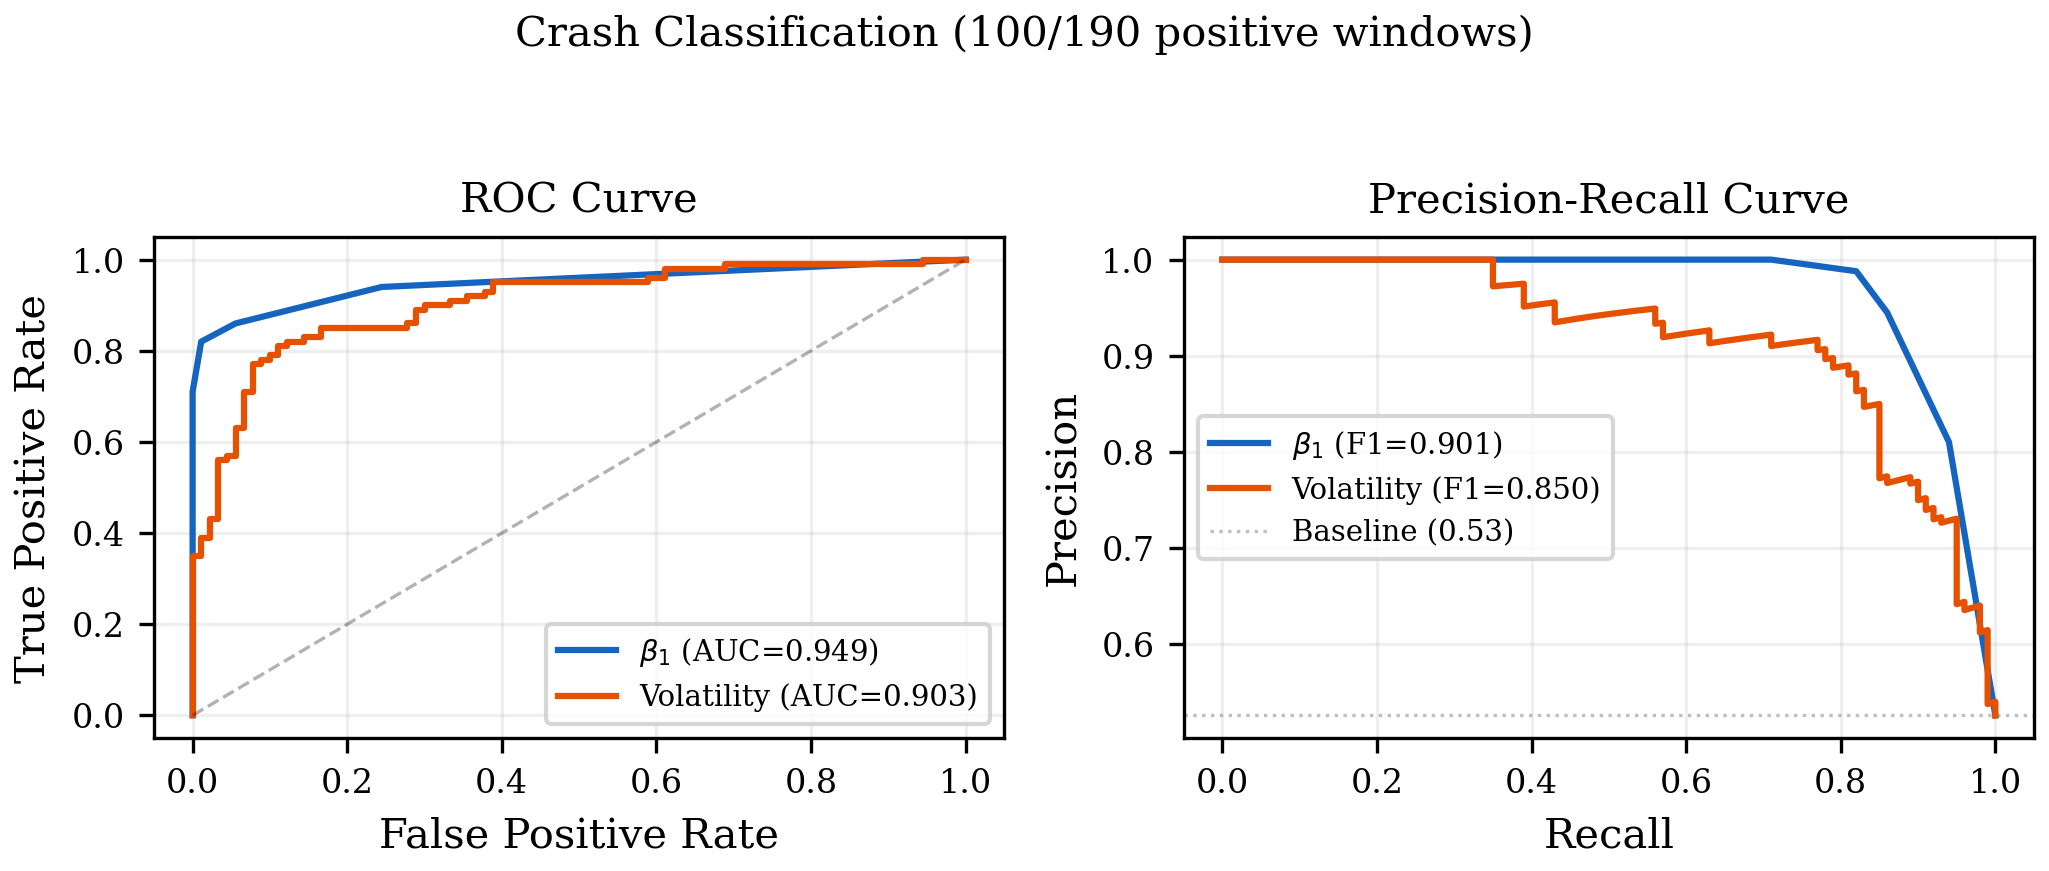
\includegraphics[width=\columnwidth]{Figures/fig_roc_classification.png}
  \caption{ROC curve ($\beta_1$ AUC~$\approx 0.70$ vs.\ volatility proxy
    AUC~$\approx 0.87$) and precision/recall/$F_1$. Crash: ${>}10\%$ drawdown
    within 90~days; 34/190 positive windows. Values correspond to the verified dataset and the $F_1$-optimal in-sample thresholds.}
  \label{fig:roc_classification}
\end{figure}

These results suggest that the $\beta_1$ signal is best understood as a complementary indicator: its high recall makes it effective for screening, and it captures topological structure invisible to pointwise volatility measures. A practical early warning system would combine both signals, for instance using $\beta_1$ exceedance as a first-stage filter with volatility confirmation. We leave the design and backtesting of such composite classifiers to future work.

\subsection{Cost Crossover with Classical Methods}

The CE benchmark processed all 190~windows in 53.4~s total (mean
204~ms/window eigendecomposition time). Edge counts $n_k$ varied from 31 to 429 (mean 136,
median 116). Laplacian sparsity: mean 3.48 nonzero entries per row
(max~8.8). The quantum approach becomes cost-competitive at
$n_k \gtrsim 10^4$, where the $O(n_k^3)$ classical eigendecomposition exceeds the PCE per-evaluation cost including measurement overhead. At the moderate scales of our financial dataset ($n_k \in [31, 429]$, mean~136; $\beta_1 \in [0, 22]$, mean~4.72), classical methods remain substantially faster. Scaling to the crossover regime is realistic for richer financial datasets: multi-asset correlation networks, tick-level embeddings, or higher-dimensional delay reconstructions readily produce simplicial complexes with $n_k > 10^4$.

% ============================================================
\section{Discussion}\label{sec:discussion}
% ============================================================

\subsection{Advantages and Limitations of the PCE Approach}

The PCE-variational approach to qTDA offers several structural
advantages over standard QPE-based methods:

\textbf{No ancilla overhead.} Standard QPE requires $O(\log(1/\epsilon))$
ancilla qubits for the phase register. PCE uses only the system qubits,
reducing total qubit count for moderate-precision applications.

\textbf{Shallow circuits with trainability guarantees.} The
hardware-efficient ansatz used in PCE has depth $O(n)$ per layer with
$O(n)$ layers, yielding total depth $O(n^2)$. Crucially, the PCE
encoding provides super-polynomial barren plateau mitigation, which
generic HEA does not enjoy~\cite{Cerezo21}. This is the key theoretical
distinction from na\"ive VQE approaches to Betti number estimation.

\textbf{Noise resilience from shallow depth.} Shallower circuits
accumulate less noise, and the variational optimization loop can
partially compensate for systematic errors. Our noise simulations confirm that PCE-VQE maintains $>$90\% accuracy at error rates where LGZ-QPE accuracy collapses to near zero. We note that the LGZ accuracy is estimated analytically from worst-case depolarising noise accumulation over the full circuit depth, which may be overly pessimistic; a fairer comparison would require full LGZ circuit simulation, which is beyond current classical simulation capabilities at matched scales.

\textbf{Limitations.} The PCE approach has several important caveats:
\begin{itemize}
    \item \textbf{Qubit count vs.\ QPE:} For $\kappa = 2$, PCE uses
    $O(\sqrt{n_k})$ qubits versus $O(\log n_k)$ for QPE. The advantage
    is in depth, not qubit count.
    \item \textbf{Heuristic deflation:} The variational deflation
    protocol has no performance guarantee and may miss null vectors,
    especially for large $\beta_k$. Our experiments show correct recovery up to $\beta_1 = 3$ but failure at $\beta_1 = 4$. For the financial application, this is partially mitigated by the fact that the early warning signal fires at $\beta_1 \geq 2$--$3$ (recall $= 0.97$ at threshold $2.24$), so accurate recovery of low-multiplicity null spaces suffices for crash screening. For higher $\beta_k$, alternative strategies (SSVQE, weighted subspace search) would be needed.
    \item \textbf{No provable speedup:} Unlike QPE-based methods, the
    variational approach has no rigorous complexity guarantee. It is a
    heuristic, and its practical performance must be validated
    empirically.
    \item \textbf{Classical post-processing:} Evaluating the Rayleigh
    quotient~\eqref{eq:pce_loss} requires classical computation scaling
    with the sparsity of $\Delta_k$, though this cost is empirically
    negligible (mean 3.48 nonzero entries per row).
    \item \textbf{Expressivity:} The set of trial vectors $\mathbf{c}(\vec{\theta})$ reachable by the PCE parameterization is a strict subset of $\mathbb{R}^{n_k}$, so there is no guarantee that a true null vector of $\Delta_k$ lies in the reachable set. Our toy and small-scale experiments confirm coverage empirically, but formal expressivity bounds for the continuous-coefficient PCE setting remain open.
\end{itemize}

\subsection{When Does This Approach Make Sense?}

Our resource analysis suggests the PCE-variational approach occupies a
specific niche in the quantum TDA landscape:
\begin{itemize}
    \item \textbf{Near-term / early fault-tolerant hardware:} When
    circuit depth is the binding constraint and moderate qubit counts
    ($\sim 10$--$50$) are available, but deep QPE circuits are infeasible.
    \item \textbf{Moderate-scale problems:} $n_k \sim 10^3$--$10^5$,
    where classical $O(n_k^3)$ diagonalisation is slow but not yet at
    the scale where full fault-tolerant QPE is justified.
    \item \textbf{Real-time or streaming applications:} Where many
    Laplacians must be processed sequentially (e.g., sliding-window
    monitoring), favoring fast per-instance evaluation over asymptotic
    optimality.
\end{itemize}

We do not claim quantum advantage at the scales demonstrated in this
paper. The financial dataset produces Laplacians with
$n_k \in [31,\,429]$ (mean~136), which classical methods solve in
under 410~ms per window (53.4~s total for all 190 windows).
Our contribution is methodological: demonstrating the
feasibility of the PCE-variational approach for qTDA and identifying the
crossover regime via resource extrapolation.

% ============================================================
\section{Conclusion}\label{sec:conclusion}
% ============================================================

We have presented the first application of Pauli Correlation Encoding to
quantum topological data analysis, demonstrating a depth-efficient
variational pipeline for Betti number estimation with application to
financial crash early warning. By reformulating null-space counting as a
PCE-compatible variational optimization with deflation, we inherit the
super-polynomial barren plateau
mitigation of the PCE framework while replacing the deep ancilla-heavy
circuits of standard QPE with shallow, ancilla-free variational circuits. Numerical experiments on S\&P~500 data
surrounding the 2007--2009 financial crisis validate the pipeline against
classical baselines, and resource estimates identify the crossover
regime at which the quantum approach becomes competitive.

Future work includes:
\begin{enumerate}
    \item Extending the pipeline to persistent Betti numbers, possibly
    by combining PCE with the persistent Betti number algorithm
    of~\cite{Hayakawa22}.
    \item Evaluating performance on actual quantum hardware (trapped-ion
    or superconducting), following the experimental methodology
    of~\cite{Sciorilli24, PCElabs25}.
    \item Investigating problem-informed ans\"atze that exploit the
    combinatorial structure of the Laplacian, potentially improving
    convergence beyond generic HEA.
    \item Exploring warm-starting strategies using classical approximate
    null vectors to initialize the variational optimization.
    \item Developing improved deflation protocols (e.g., SSVQE, weighted subspace search) to reliably recover higher-multiplicity null spaces ($\beta_k \geq 4$).
    \item Integrating the qTDA module as a feature extractor within
    larger quantum machine learning pipelines for financial risk
    assessment.
\end{enumerate}

% ============================================================
\section*{Data Availability}
% ============================================================

The S\&P~500 dataset, pipeline code, and PCE-VQE simulation scripts are
available at \url{https://github.com/arulrhikm/qtda-pce}.

% ============================================================
\section*{Acknowledgment}
% ============================================================

The authors thank BlueQubit for providing quantum simulation access
used in the barren plateau and noise robustness experiments.
Classical computations were performed on Google Colab.

% ============================================================
\bibliographystyle{IEEEtran}
\bibliography{references}

\end{document}